\documentclass[10pt,a4paper,openany]{article}

\usepackage[english,italian]{babel} %lingue utilizzabili


%PER GRAFICA
\usepackage{graphicx}
\usepackage{fancyhdr} %per intestaz e piè di pagina
\usepackage{subfig}
\usepackage{float}
\usepackage{caption}


\usepackage[utf8]{inputenc} %codifica e input

\usepackage{hyperref} %indice linkato ai paragrafi di riferimento
\hypersetup{
  colorlinks,
  citecolor=gray,
  filecolor=brown,
  linkcolor=black,
  urlcolor=cyan
}

\usepackage{lastpage} %per sapere il numero di pagine totali

\usepackage{parcolumns} %testo affiancato in colonna

\usepackage{verbatim}%commenti a blocchi
\usepackage{listings} %Per inserire codice
\usepackage[usenames]{color} %Per permettere la colorazione dei caratteri 

\usepackage[a4paper,top=3cm,bottom=2cm,left=2cm,right=2cm] {geometry} %imposta pagina formato A4 e setta margini a piacimento
\usepackage[pdftex]{lscape} %per settare pagine in landscape

\renewcommand{\familydefault}{\sfdefault}   %mette tutto il carattere con uno stile ''grazioso''

\definecolor{editorGray}{rgb}{0.95, 0.95, 0.95}
\definecolor{editorOrange}{rgb}{1, 0.5, 0} % #FF7F00 -> rgb(239, 169, 0)
\definecolor{editorGreen}{rgb}{0, 0.6, 0} % #007C00 -> rgb(0, 124, 0)




%personalizzazione classe per il codice XML
\lstnewenvironment{xml}[1][] 
{\lstset{basicstyle=\scriptstyle \ttfamily, columns=fullflexible, keywordstyle=\color{blue}\bfseries, ndkeywordstyle=\color{blue}\bfseries , ndkeywords={references}, numberstyle=\color{red}, commentstyle=\color{editorGreen}, showstringspaces=false, stringstyle=\color{editorOrange},
language=XML, basicstyle=\small,
numbers=left, numberstyle=\tiny,
tabsize=2, stepnumber=10, numbersep=5pt, breaklines=true, frame=single, rulecolor=\color{black}, #1}}
{\lstset {language=XML,morekeywords={xml}}}{}


%personalizzazione classe per il codice HTML
\lstnewenvironment{html}[1][] 
{\lstset{basicstyle=\scriptstyle \ttfamily, columns=fullflexible,
keywordstyle=\color{blue}\bfseries, ndkeywords={content,=,charset=, id=, width=, height=},	 ndkeywordstyle=\color{editorGreen}\bfseries , numberstyle=\color{red} commentstyle=\color{red}, showstringspaces=false, stringstyle=\color{editorOrange},
language=HTML, basicstyle=\small,
numbers=left, numberstyle=\tiny,
tabsize=2, stepnumber=10, numbersep=5pt, breaklines=true, frame=single, rulecolor=\color{black}, #1}}{}

%personalizzazione classe per il codice C++
\lstnewenvironment{CPP}[1][] 
{\lstset{basicstyle=\scriptstyle \ttfamily, columns=fullflexible,
keywordstyle=\color{blue}\bfseries, ndkeywords={content,=,charset=, id=, width=, height=},	 ndkeywordstyle=\color{editorGreen}\bfseries , numberstyle=\color{red} commentstyle=\color{red}, showstringspaces=false, stringstyle=\color{editorGreen},
language=C++, basicstyle=\small,
numbers=left, numberstyle=\tiny,
tabsize=2, stepnumber=10, numbersep=5pt, breaklines=true, frame=single, rulecolor=\color{black}, #1}}{}


%%%%%%%%%%%%%%%%%%%%%%%%%%%%%%%%%%%%%%%%%%%%%%%%%%%%%%%%%%%%%%%%%%%%
%%%%%%%%%%%%%%%%%%%%%%%%%%%%%%%%%%%%%%%%%%%%%%%%%%%%%%%%%%%%%%%%%%%%
%%%%%%%%%%%%%%%%%%%%%%%%%%%%%%%%%%%%%%%%%%%%%%%%%%%%%%%%%%%%%%%%%%%%


\begin{document}

\begin{figure}
\centering

\includegraphics[angle=0,scale=.30]{LOGO.png}
\end{figure} 


\title{ \textbf{\huge PROGRAMMAZIONE AD OGGETTI}\vspace{0.7cm} \\ {\Huge Relazione del progetto} \vspace{0.3cm} \\ {\Large Anno accademico 2015/2016} }
%\date{}
 
\author{\textbf{Zecchin Giacomo (1070122)}}

\maketitle
\thispagestyle{empty}


%da qui stile intestazione e piè di pagina cosi definiti
\pagestyle{fancy}
\lhead{}
\rfoot{\vspace {1pt} Relazione del progetto}
\cfoot{\vspace{1pt} Pagina: \thepage\ di \pageref{LastPage}}
\fancyfoot[L]
	{\vspace{1pt}
   		\hyperref[sec:index] {
\includegraphics[scale=0.06]{leftfoot.png}} % icona linkata all'index
	 }
\renewcommand{\footrulewidth}{0.5pt}


\tableofcontents \label{sec:index} %CREA INDICE LINKABILE


\newpage


\section{Scopo del progetto}

Mediary è il risultato di questo progetto per il corso di programmazione ad oggetti che aveva come scopo quello di creare un applicativo sviluppato in C++/Qt.\\\\
L'applicazione intende rappresentare uno spazio personale nel quale annotare tutte le serieTv o i film già visti, preferiti oppure col desiderio di vedere in futuro.\\
Mediary consente quindi di accedere singolarmente come utente per aggiungere nuovi \textit{media} al proprio diario (\textit{diary}).\\
L'unione di queste due parole, \textbf{Media} e \textbf{Diary}, va difatti a creare il nome dell'applicazione.\\\\
Il progetto è semplice ma allo stesso tempo funzionale, diretto e comprensibile per l'utente; vediamo nel seguito tutte le funzionalità.\vspace{20pt}



\section{Funzionalità offerte}
	\subsection{Utenti}

	Avviata, l'applicazione presenta subito una finestra centrale per l'inserimento diretto dei dati necessari ad effettuare il \textbf{login} ed 
	accedere  immediatamente all'area personale.\\
	In alternativa, se non si possiedono già delle credenziali, è presente un bottone per la \textbf{registrazione} poco più in basso, che farà entrare nella 
	finestra dedicata alla creazione di un nuovo utente.
	In entrambi questi due casi sono presenti dei controlli di consistenza dei dati descritti più approfonditamente nella sezione *sez.* .\\
	E' comunque data la possibilità di \textbf{modificare i propri dati} in un secondo momento.
		
	\subsection{Media}
	
	Le funzionalità offerte per i media sono invece quelle di \textbf{creazione, modifica, visualizzazione per tipo ed eliminazione}. (In 
	dettaglio qui *sez*)\vspace{20pt}
	

\section{Schema Logico}	

Il \textit{Design Pattern} utilizzato per la progettazione è il classico pattern \textbf{MVC} separando quindi il \textit{Model} dalla \textit{View} con l'ausilio due classi che formano il \textit{Controller}.

Vediamo nelle sottosezioni seguenti le tre componenti e le classi che li compongono.\\\\\\

%%%%%% Per mettere a sinistra la caption sennò rimane al centro%%%
%\captionsetup{
 % justification=raggedright,
  %singlelinecheck=false
%}

\begin{figure}[!h]
\centering
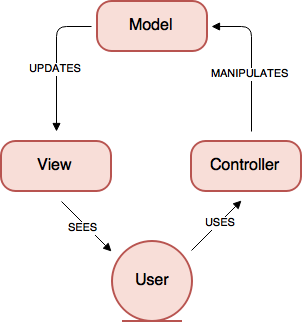
\includegraphics[angle=0,scale=.45]{MVC.png}\\
\caption{Interazione nel pattern MVC}
\label{fig:MVC}
%\hspace{1in}
\end{figure}


\newpage

	\subsection{Model}
	
	Di seguito tutte le entità che vanno a formare la parte del \emph{MODEL} del progetto.
	
		\subsubsection{Gerarchia polimorfa}
	
		La \textbf{gerarchia G polimorfa} che contribuisce a formare il modello dati del progetto è composta dalle classi:
	
		\begin{itemize}
	
			\item \textbf{Media}: E' la \underline{classe base astratta} della gerarchia polimorfa contenente i campi dati \texttt{title, year, 
			creationDate }e \texttt{changeDate} comuni a tutte la classi derivate.
			All'interno è dichiarato il metodo \textit{virtuale puro} 
			\begin{CPP}
			virtual void saveMedia(QXmlStreamWriter& xmlWriter) const=0;
			\end{CPP}		 
			per eseguire il \textbf{salvataggio POLIMORFO dei media} nel mediaDatabase.xml .
			ed il metodo \textit{virtuale puro}
			\begin{CPP}
			virtual QString getType() const=0;
			\end{CPP}
			che \textbf{ritorna il tipo POLIMORFO del media} quando si carica la tabella per visualizzarli tutti nella view apposita (descrizione più avanti nella View).
			\item \textbf{SerieTV}: E' una \underline{classe concreta derivata pubblicamente} dalla base perché implementa il metodo virtuale puro della base.\\
		 	Contiene i campi dati privati aggiuntivi caratteristici di una serieTv \texttt{descriptionEp, season, numberEp, lenghtEp} rappresentanti in ordine 
			descrizione, numero della stagione dell'ep., numero episodio e lunghezza in minuti.
		 	\item \textbf{Film}: E' una \underline{classe concreta derivata pubblicamente} dalla base perché implementa il metodo virtuale puro della base.\\
		 	Contiene i campi dati privati aggiuntivi caratteristici di un film \texttt{plot, distribution, duration} rispettivamente trama, casa di produr./distribuzione e 
			durata in ore:minuti del film.
	
		\end{itemize}
	
		\subsubsection{Il contenitore}
	
		\textbf{Container.h} è una \underline{classe esterna alla gerarchia G} che contiene la \textbf{definizione completa di un opportuno contenitore C}, con relativi 
		\textbf{iteratori}, che permettono inserimenti, rimozioni e modifiche.\\\\
		Il contenitore C è dal punto di vista progettuale un \textbf{template di classe} (perciò definito completamente in un unico file header) con due classi 
		\textbf{Nodo} e \textbf{Smartp} annidate ed un unico campo dati \texttt{Smartp first} nella sua \underline{parte privata.}\\\\
		Smartp ha come unico campo dati un \texttt{Nodo* punt} mentre la classe Nodo ha 3 campi dati \texttt{T info; Smartp next; int riferimenti}.\\\\
		Nella parte pubblica di Container è definita la classe annidata \emph{Iterator} con un campo dati privato \texttt{Smartp punt} per accedere agli elementi nel 
		contenitore.\\
		Le classi \emph{Container} ed \emph{Iterator} sono infatti \underline{reciprocamente amiche}.\\\\
		\emph{Iterator} \textbf{ridefinisce gli operatori} di incremento (post e prefisso), dereferenziazione, uguaglianza e disuguaglianza per modificare gli elementi, 
		mentre \emph{Container} ha i vari metodi di push e pop per manipolare la lista e begin(), end() e la ridefinizione dell'operatore di indicizzazione che usano 
		Iterator.
		
		\subsubsection{Classe User}
		
		E' una \underline{classe concreta esterna a G} che rappresenta l'entità utente per accedere all'applicazione.
		
		I suoi campi dati sono: \texttt{username, password, name, surname} ed infine un c.d. \texttt{Container<const Media*> mediaDatabase;} che rappresenta il 
		contenitore di tutti i media appartenenti allo \emph{User}.
		
		\subsubsection{Classe Database}
		
		E' una \underline{classe concreta esterna a G} che rappresenta il database degli utenti di Mediary ed ha infatti come suo unico campo dati privato il campo
		\texttt{Container<const User*> userDatabase;} .
	
		\begin{figure}
			\centering
			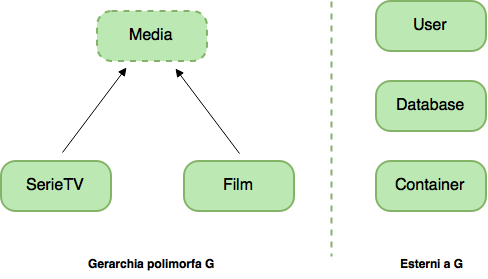
\includegraphics[angle=0,scale=.45]{Model.png}\\
			\caption{Entità che compongono il Model}
			\label{fig:Model}
		\end{figure}\vspace{20pt}


\newpage
	
	
	\subsection{View}
	
	L'intera \emph{VIEW} è rappresentata da una \textbf{gerarchia polimorfa} che fa capo alla \underline{classe base astratta} \textbf{MainView} .
	Essa deriva pubblicamente a sua volta dalla cl.astratta di Qt \emph{QWidget} .\\\\
	In \emph{MainView} è definito il metodo \textit{virtuale puro} 
	\begin{CPP}
		virtual void loadGraphic() =0;
	\end{CPP}
	che permette di \textbf{caricare la view POLIMORFA} corretta in base al tipo dinamico del puntatore della classe derivata.
	
		\subsubsection{Classi e gerarchia }

	Le classi derivate da \emph{MainView} sono:
	\begin{itemize}
		\item \textbf{loginView}: E' la classe che si preoccupa di costruire la view di start all'avvio dell'applicazione.
		\item \textbf{userView}: E' la classe che costruisce la view per uno User. Ci si accede una volta eseguita correttamente l'autenticazione in loginView.
		\item \textbf{serietvView}: E' la classe che costruisce la view di una SerieTV. Viene creata a partire dalla \emph{userView} quando si vuole creare o modificare 
		una SerieTV.
		\item \textbf{filmView}: E' la classe che costruisce la view di un Film. Viene creata a partire dalla \emph{userView} quando si vuole creare o modificare 
		un Film.
		\item \textbf{userDataView}: E' la classe che costruisce la view per vedere/modificare i dati di uno User. Vi si accede sempre dalla \emph{userView} quando
		si clicca nel bottone dedicato.
		\item \textbf{registrationView}: E' la classe che costruisce la view per la registrazione di un nuovo User.  In alternativa al login cliccando nel bottone per la 
		registrazione si accede ad essa.
		\item \textbf{dialogMessage}: E' una classe per la rappresentazione di una finestra che da una view di dialogo con l'utente, composta da un titolo, un 
		messaggio ed un bottone che se cliccato è collegato alla chiusura della finestra stessa. \emph{dialogMessage} deriva pubblicamente dalla classe di Qt 
		\emph{QDialog} .
	\end{itemize}
		
		\newpage
		
		
		\begin{figure}[!h]
			\centering
			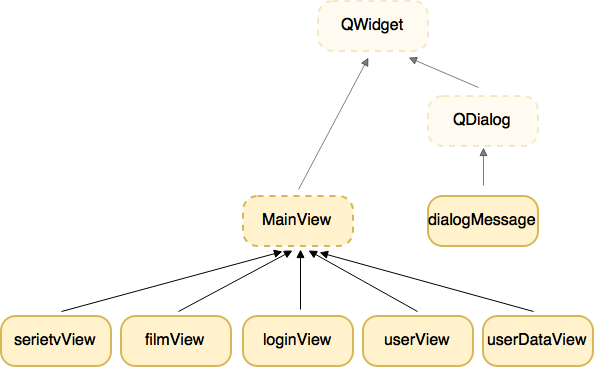
\includegraphics[angle=0,scale=.45]{View.png}\\
			\caption{Gerarchia della View}
			\label{fig:View}
		\end{figure}
	
		\subsubsection{Presentazione}
		
		All'avvio di Mediary si apre la view di login; in alto a destra è presente il bottone \textit{esci} per chiudere il programma.\\
		Nel caso si eseguisse con successo la procedura di l'autenticazione cliccando nel login button si verrebbe mandati alla finestra personale con la possibilità di 
		aggiungere, modificare oppure eliminare media.

		Nel mezzo della \emph{userView} è presente una tabella che permette di visualizzare, in ordine di inserimento dal più al meno recente, i media divisi per 
		serieTv, film oppure tutti i tipi (l'opzione è selezionabile tramite una comboBox).

		E' possibile modificare un elemento cliccando al di sopra \textbf{titolo} del media che si intende manipolare, mentre per cancellarlo è necessario cliccare sopra 
		l'icona del cestino nell'ultima colonna della tabella corrispondente alla riga del media (si aprirà un avviso per la conferma).

		La stessa finestra offre inoltre la possibilità di modificare i propri dati personali cliccando nel bottone ''Gestisci dati utente''.

		Ogni finestra per la manipolazione dei dati del model ha i suoi controlli di consistenza dei dati.\\
		Infine, nella parte più bassa della view utente c'è un bottone per il logout che riporta alla \emph{loginView} con la possibilità di entrare in quella per la 
		registrazione.
		
		\begin{comment}
		\begin{figure}[!h]
			\centering
			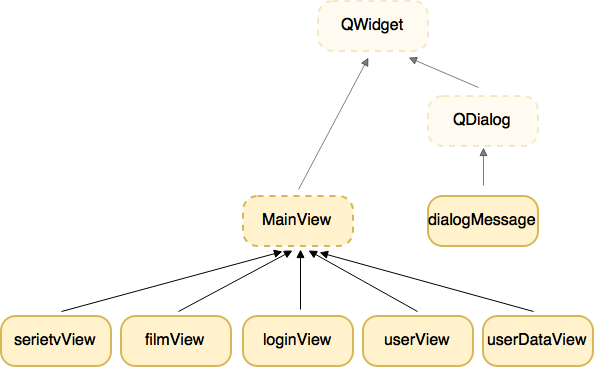
\includegraphics[angle=0,scale=.45]{View.png}\\
			\caption{Gerarchia della View}
			\label{fig:View}
		\end{figure}
		\end{comment}
	
	\newpage
	
		\subsection{Controller}
		
		Il \emph{CONTROLLER} è composto da sole due classi che però riescono a gestire ordinatamente tutte le funzioni e le view del programma:
		
			\subsubsection{mediaryController}
			
			Nel \emph{main} del programma si crea subito un oggetto \texttt{controller} di tipo \emph{mediaryController} che costruisce subito la 
			\emph{loginView}.
			Nel caso in cui l'utente effettui il login viene chiamata la funzione \texttt{verifyLogin(..)} che in caso positivo permette l'apertura della \emph{userView}
			personale passando la gestione allo \emph{userController}.\\\\
			In caso differente chiama la funzione \texttt{openRegistrationView()} che costruisce la view di registrazione.
			
			\subsubsection{userController}
			
			Questa classe connette le restanti funzionalità che sono accessibili una volta entrati nella view personale, ovvero quelle di \textbf{creazione, modifica, 
			cancellazione dei media, la gestione dei propri dati ed il logout.}
			
\section{Database}

\newpage

I dati reali 





%\selectlanguage{italian}	%inserirlo causerebbe errore in compilazione per lettere accentate-->non risolto


	
%per inserire un'immagine:

%\begin{landscape}
%\begin{figure}
%\subsection{Schema E-R iniziale del database}
%\centering
%\includegraphics[angle=0,scale=.40]{image.jpg}
%\hspace{1in}
%\label{schema}
%\caption{schema E-R}
%\end{figure}
%\end{landscape}



%inserire codice c++:

%\begin{CPP}
%#include <iostream>
%\end{CPP}







\end{document}
